\documentclass{scrbook}
\usepackage{graphicx} % Required for inserting images
\usepackage{tabularx} % Required for fixed width tables
\usepackage{scrlayer-scrpage} % Required for the subtitles
\usepackage{url} % Required for the URLs
\usepackage{hyperref} % Required for the URLs
\usepackage{listings} % Required for the code snippets
\usepackage{mathtools} % Required for the system of equations
\usepackage{amsmath,amssymb} % Required for some math symbols
\usepackage{enumitem} % Required for lettered lists

\usepackage{fontspec}
\setmonofont{DejaVu Sans Mono} % Overleaf has this font pre-installed

\usepackage{subcaption} % To use subfigures

% Put the caption of the snippets at the bottom
\lstset{
    captionpos=b
}


\title{Blockchain Hyperledger and IOTA}
\subtitle{Ambient intelligence course (A.Y. 2025/2026)\\Topic taught by Prof. Arnaldo Tomasino}
\author{Gabriele Colapinto}
\date{\today}

\begin{document}

\maketitle
\thispagestyle{empty}

{\Large\textbf{License}} \\
{Notes from Ambient intelligence (A.Y. 2025/2026) by Gabriele Colapinto. 
Course taught by professors Michele Ruta, Floriano Scioscia, Arnaldo Tomasino, Davide Loconte — 
Licensed under CC BY-NC 4.0.\\
\url{https://creativecommons.org/licenses/by-nc/4.0/}}

\vspace*{\fill}
\rule{\textwidth}{0.2pt}
\small{© 2025 Gabriele Colapinto \\
Released under the \href{https://creativecommons.org/licenses/by-nc/4.0/}{Creative Commons Attribution–NonCommercial 4.0 International License}}

\clearpage

\tableofcontents

\chapter{Fundamental Definitions and Technological Foundations}

The Fourth Industrial Revolution, or Industry 4.0, represents a paradigm shift where production systems are no longer isolated silos but interconnected, digital ecosystems driven by massive data streams from integrated sensors and actuators. However, a critical strategic bottleneck persists: a systemic "lack of trust" between independent market players. This lack of confidence hinders essential data exchange and prevents "spillover effects"—the positive network externalities where regional proximity and knowledge sharing between companies drive collective innovation and growth. Distributed Ledger Technology (DLT) is uniquely positioned to resolve this by providing a decentralized infrastructure that ensures transparency, security, and data integrity without the need for a central intermediary (see table \ref{tab:database_dlt_comparison}).\\

DLT functions as a geographically decentralized database synchronized across a network of stakeholders (nodes). Its architectural integrity rests on four pillars derived from the source:
\begin{itemize}
    \item \textbf{Decentralization:} Eliminating single points of failure by distributing and synchronizing data across all nodes.
    
    \item \textbf{Encryption and Hashing:} Production data is secured via cryptographic signatures. A "hash" ensures that the information is tamper-evident; any modification to the underlying data radically alters the hash value, exposing the intervention.
    
    \item \textbf{Consensus Algorithms:} These mechanisms require nodes to agree on the database’s current state. This agreement is often tied to economic or participatory incentives, ensuring that no state transition occurs unnoticed.
\end{itemize}

\begin{table}[]
    \centering
    \begin{tabularx}{\linewidth}{|X|X|X|}\hline
         \textbf{Feature} & \textbf{Traditional Databases} & \textbf{Distributed Ledgers}\\
         \hline

        \textbf{Control} & Centralized authority manages data. & Geographically decentralized across nodes.\\
        \hline

        \textbf{Integrity} & Records can be modified or deleted by admins. & Tamper-proof; reveals any attempt at manipulation.\\
        \hline

        \textbf{Traceability} & Limited to internal logs. & Full immutable history of all transactions.\\
        \hline

        \textbf{Intermediaries} & Required for trust/verification. & Eliminated; trust is algorithmic and protocol-based.\\
        \hline

        \textbf{Data Exchange} & Restricted by silos and trust deficits. & Facilitates secure, peer-to-peer (P2P) exchange.\\
        \hline
         
    \end{tabularx}
    \caption{Comparison between a traditional database and a distributed ledger technology}
    \label{tab:database_dlt_comparison}
\end{table}

\textbf{The "So What?" Layer:} From an architectural perspective, it is vital to understand that DLT does not inherently guarantee the correctness of data (the "garbage in, garbage out" principle); rather, it guarantees the \textit{unmanipulated state} of that data once recorded. By providing this "network of trust", DLT transforms internal data from a mere byproduct of manufacturing into a high-value, tradable commodity. This enables a "data economy" where information can be monetized and shared to capture the spillover effects previously stifled by security concerns.\\

While these foundational features are universal, their industrial application bifurcates into two distinct topologies: the structured, permissioned architecture of Hyperledger Fabric (a product of the Hyperledger foundation, see figure \ref{fig:hyperledger_products}) and the lightweight, probabilistic nature of IOTA.

\begin{figure}
    \centering
    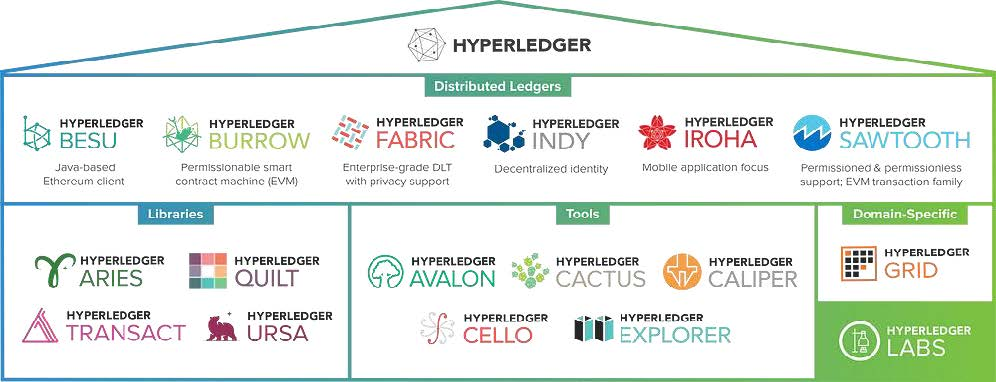
\includegraphics[width=\linewidth]{Images/Products of the Hyperledger foundation.jpg}
    \caption{Products of the Hyperledger foundation (The Linux Foundation)}
    \label{fig:hyperledger_products}
\end{figure}

\chapter{Hyperledger Fabric: A Permissioned DLT for Business Ecosystems}

Hyperledger Fabric is a permissioned blockchain platform hosted by the Linux Foundation, engineered to meet the demands of enterprise applications. Its strategic importance lies in its ability to provide privacy, modularity, and granular control over network participation, making it ideal for complex business ecosystems where trust and confidentiality are paramount.\\

As a permissioned platform, participation in a Hyperledger Fabric network is not open to the public. Every participant, whether a user, a peer node, or an application, must possess a recognized identity within the network. This identity is established through cryptographic materials, such as digital certificates, ensuring that only verified and authorized entities can interact with the ledger.

\section{Core Features and Architecture}

Hyperledger Fabric's design is grounded in several foundational features that enable its deployment in sophisticated, multi-party business environments.

\begin{itemize}
    \item \textbf{Modular Structure:} The platform achieves high scalability and resilience through a design built on plug-and-play modules. This allows organizations to construct a network that accommodates advanced business ecosystems by including necessary functionalities while excluding others, depending on the specific deployment context.
    
    \item \textbf{Pluggable Implementations:} Fabric offers significant flexibility by allowing key components to be swapped. This includes the ability to configure different consensus mechanisms, such as \textbf{Raft} for production environments or \textbf{Solo} for development purposes. Similarly, data storage options for ledger components can be customized to meet specific needs.
    
    \item \textbf{Privacy and Permissions:} Granular control over access and data confidentiality is a core tenet of the platform. Permissions are enforced using \textbf{Membership Service Providers (MSPs)}, which manage user identities and roles. Furthermore, \textbf{private channels} allow a subset of network participants to create a confidential ledger, ensuring that sensitive transactions are only visible to the authenticated parties involved.
\end{itemize}

\section{Key Components of the Fabric Network}

A Hyperledger Fabric network is composed of several primary components that work in concert to maintain a secure and consistent distributed ledger.

\begin{itemize}
    \item \textbf{Ledger (L):} The ledger in Fabric is comprised of two distinct but related parts.
    \begin{enumerate}
        \item \textbf{Log of Transactions:} This is the traditional, immutable chain of blocks that provides a tamper-evident record of all state changes. Each block within this log represents a specific state transition.
        \item \textbf{World State (W):} This component functions as a database that maintains the current value of the ledger's state at any given time. It is typically implemented as a key-value store, offering two primary options: \textbf{LevelDB} (the default) or \textbf{CouchDB} (which supports more advanced, rich queries).
    \end{enumerate}
    
    \item \textbf{Peer (P):} Peers are the fundamental network nodes that maintain copies of the ledger and the world state. They are also responsible for hosting and executing the smart contracts, known as chaincode, that govern the network's business logic. Peers host ledgers and chaincode and are responsible for creating and endorsing transactions.
    
    \item \textbf{Ordering Service (O):} This component is responsible for the consensus mechanism. It accepts endorsed transactions, orders them into a consistent sequence, packages them into blocks, and then distributes these blocks to all peers in the channel. It is crucial to understand that an ordering node (which provides the ordering service) is not a node which has all the functionalities of a peer with the additional functionalities of transaction ordering, packaging into a block and distributing the block to the peers. \textbf{Ordering nodes are not a sort of super-peers!} They are only responsible for arranging the transaction into blocks and distributing them to the peers.
    
    \item \textbf{Channel (C):} A channel is a private blockchain overlay that provides data isolation and confidentiality within the broader Fabric network. All transacting parties must be authenticated to a specific channel to interact with its ledger. Each channel maintains a completely separate ledger, ensuring that data is only shared among the designated channel members.
\end{itemize}

\section{Membership and Identity Management}

Hyperledger Fabric employs a sophisticated system for managing identities and permissions, ensuring that only authorized participants can perform specific actions on the network.

\begin{itemize}
    \item \textbf{Certificate Authority (CA):} The CA is the component responsible for issuing X.509 digital certificates. These certificates are used to cryptographically link an identity (such as a peer node or a client application) to a specific organization, forming the basis of trust in the network.

    \item \textbf{Organization (R):} An organization is a member of the private blockchain network. It can represent any entity, from a large multinational corporation to a small business or even an individual. Each organization manages the identities of its affiliated components.

    \item \textbf{Membership Service Provider (MSP):} The MSP is an abstract component that defines the rules by which identities are validated, authenticated, and assigned permissions. In Hyperledger Fabric, identity management is not hierarchical but based on cryptographic trust (i.e., certificates issued by trusted Certification Authorities). MSPs operate at multiple levels:

    \begin{enumerate}
        \item \textbf{Local MSPs:} These reside on the file system of a specific node (peer or orderer) and define the permissions for that actor. A Local MSP contains the cryptographic material (certificates, private keys, root CAs) used by the node to:
        \begin{itemize}
            \item authenticate itself to the network,
            \item sign transactions,
            \item define local administrative roles.
        \end{itemize}
        Each node has its own Local MSP, but multiple nodes of the same organization share a common root of trust (i.e., the same CA).
    
        \item \textbf{Organization MSPs (``Global MSPs''):} An Organization MSP represents an entire organization at the channel level. It defines:
        \begin{itemize}
            \item which Certification Authorities are trusted,
            \item how identities belonging to the organization are validated,
            \item which roles (admin, client, peer) are recognized.
        \end{itemize}
    
        All nodes (peers/orderers) belonging to the same organization have Local MSPs that are \textbf{consistent with} the Organization MSP, meaning that their certificates are issued by the trusted CAs defined in it.\\
    
        There is no direct communication between Local MSPs and the Organization MSP. Instead, they are linked by a shared root of trust.
    
        \begin{center}
        \begin{verbatim}
                    CHANNEL MSP
            ┌────────────────────────┐
            │ MSP ORG1 (CA1, rules)  │
            │ MSP ORG2 (CA2, rules)  │
            └────────────────────────┘
                     ↑
                     | (identity validation)
    
         ┌───────────────┐     ┌───────────────┐
         │ Peer P1 (ORG1)│     │ Peer P2 (ORG1)│
         │ Local MSP     │     │ Local MSP     │
         │ (cert CA1)    │     │ (cert CA1)    │
         └───────────────┘     └───────────────┘
        \end{verbatim}
        \end{center}
    
        Therefore, a node is recognized as part of an organization if its identity satisfies the rules defined in the Organization MSP.
    
        \item \textbf{Channel MSP:} The Channel MSP is the identity configuration shared across all nodes participating in a channel. It is defined in the channel configuration and replicated on every peer and ordering node.\\
    
        Structurally, the Channel MSP is not a single MSP but a \textbf{collection of Organization MSPs}, one for each organization participating in the channel:
    
        \begin{center}
        \begin{verbatim}
                    Channel MSP
            ┌───────────────────────┐
            │ MSP ORG1              │
            │ MSP ORG2              │
            │ MSP ORG3              │
            └───────────────────────┘
        \end{verbatim}
        \end{center}
    
        The Channel MSP is used to:
        \begin{itemize}
            \item authenticate all channel participants,
            \item enforce channel-wide policies (e.g., endorsement policies, access control),
            \item enable trust among independent organizations.
        \end{itemize}
    
        The Channel MSP configuration is kept consistent across the network through the \textbf{consensus protocol}, which ensures that all nodes observe the same sequence of configuration updates.\\
    
        \textbf{Important clarification:}
        \begin{itemize}
            \item Changes to the Channel MSP (e.g., adding/removing an organization, updating an Organization MSP, or changing trusted CAs) are not autonomously broadcast by a single node.
            \item Instead, they are introduced as \textbf{configuration update transactions}.
            \item These transactions must satisfy the channel policies (e.g., be signed by required administrators), and are then:
            \begin{enumerate}
                \item ordered by the ordering service,
                \item included in a configuration block,
                \item distributed to all peers.
            \end{enumerate}
        \end{itemize}
    
        Therefore, the consensus protocol does not simply "notify" nodes, but guarantees that all nodes agree on and apply the same configuration changes in a consistent order.
    
    \end{enumerate}

\end{itemize}

\subsection{Hyperledger Fabric network example}

\begin{figure}[htbp]
    \centering
    \begin{subfigure}[b]{0.65\linewidth}
        \centering
        
\includegraphics[height=6cm]{"Images/Network example.jpg"}
    \end{subfigure}%
    \hfill
    \begin{subfigure}[b]{0.2\linewidth}
        \centering
        
\includegraphics[height=6cm, keepaspectratio]{"Images/Network example legend.jpg"}
    \end{subfigure}%
    \caption{Example of Hyperledger Fabric network (left) and legend of the components (right)}
    \label{fig:hyperledger_fabric_network_example}
\end{figure}

Figure \ref{fig:hyperledger_fabric_network_example} shows a simple example of a peer node and an ordering node participating in the same channel within a Hyperledger Fabric network. To understand the picture, it is convenient to start from its center. The peer node and the ordering node are connected to the channel (the connection is represented by solid lines). The channel is a logical construct that defines a shared communication context and a common ledger among participating nodes.\\

The remaining elements describe how identities and trust are managed. Membership Service Providers (MSPs) are linked to components through dashed lines, representing logical relationships rather than physical connections. In particular, a node (peer or orderer) is associated with a Local MSP, which contains the cryptographic material (certificates and keys) used by the node to authenticate itself and sign transactions.\\

At the channel level, the set of Organization MSPs (sometimes referred to as ``global MSPs'') forms the Channel MSP. Each Organization MSP defines how identities belonging to a specific organization are validated (e.g., by specifying trusted Certification Authorities). Therefore, organizations are recognized in the channel based on the validation rules defined in their MSPs.\\

In the bottom right corner of the figure, the Organization~1 MSP is shown in association with the network. This representation may be misleading, as it could suggest that only one organization is identified in this way. In reality, every organization participating in the channel is represented by its own MSP within the Channel MSP, which defines how its identities are validated by the other nodes of the network.\\

Finally, Certification Authorities (CAs) are depicted outside the shaded area because they are not part of the blockchain network itself. They belong to the Public Key Infrastructure (PKI) and are responsible for issuing X.509 certificates that define the identities of nodes and users. The arrows between MSPs and CAs indicate that the identities contained in the MSPs are issued and signed by the corresponding Certification Authorities.

\subsection{Hyperledger Fabric transaction lifecycle}

\begin{figure}[htbp]
    \centering
    \begin{subfigure}[c]{0.5\linewidth}
        \centering
        
\includegraphics[height=4.5cm, keepaspectratio]{"Images/Transaction lifecycle.jpg"}
    \end{subfigure}%
    \hfill
    \begin{subfigure}[c]{0.4\linewidth}
        \small{
            \vspace{0pt}
            Legend:
            \begin{itemize}
                \item A = Client application
                \item CA = Certification Authority
                \item R = Organization
                \item P = Peer node
                \item O = Ordering node
                \item C = Channel
                \item CC = Channel configuration (network configuration)
                \item S = Step (S5 = Step 5)
                \item L = Ledger (L1 = Ledger 1)
            \end{itemize}
        }
    \end{subfigure}%
    \caption{Example of Hyperledger Fabric transaction life cycle (left) and legend of the components (right)}
    \label{fig:hyperledger_fabric_transaction_lifecycle}
\end{figure}

Figure \ref{fig:hyperledger_fabric_transaction_lifecycle} depicts an example of the Hyperledger Fabric transaction lifecycle, which is composed of the following steps:
\begin{enumerate}
    \item The client application sends a transaction proposal to the endorsing peers.
    \item The peers execute the smart contract (chaincode) and return endorsement responses, including the read/write set.
    \item The client collects the endorsements and, if they satisfy the endorsement policy, sends the transaction to the ordering service.
    \item The ordering node orders transactions into a block and distributes the block to the peers on the channel.
    \item The peers validate the transactions in the block and commit them to their local copy of the ledger.
\end{enumerate}

The key to understanding the picture is to consider colors: all entities related to Organization 0 (the one owning the ordering node) are green, those related to Organization 1 are pink, and those related to Organization 2 are gray.\\

In the figure, the organizations are represented close to the channel configuration because it contains the definition of the organizations and their roles in the network. The dotted line connecting the channel configuration to the channel represents the fact that interactions on the channel are governed by the policies defined in the configuration.\\

Certification Authorities are depicted outside the Hyperledger Fabric network because they are part of the Public Key Infrastructure and are responsible for issuing identities and certificates for entities such as nodes, users, and administrators. Client applications are also external entities that interact with the network but are not part of it.\\

In this scenario, Organization 1 uses its client application to invoke a gRPC call to the gateway service of a peer (P1) in order to execute a smart contract (chaincode). The execution produces an endorsement response, including the read/write set, which is sent back to the client. The client then collects endorsements from the required peers (e.g., P2) and submits the endorsed transaction to the ordering service. The ordering service packages the transaction into a block and distributes it to all peers in the channel. Upon receiving the block, peers validate the transactions and commit them to their local copy of the distributed ledger (L1) in the final step of the transaction lifecycle (S5).

\section{Smart Contracts (Chaincode) and Endorsement}

In Hyperledger Fabric, smart contracts encapsulate the network's business logic and are deployed in a package called \textbf{chaincode}.\\

Chaincode execution is triggered by transaction requests from authenticated external applications. When executed, chaincode can interact with the world state to query or update ledger data. Fabric provides robust language support for chaincode development, including \textbf{Go}, \textbf{Node.js}, and \textbf{Java}.\\

There are two primary models for deploying chaincode: the default method where it runs in a container on the peer, and an external deployment model that allows chaincode to run as an independent service.\\

A critical concept in Fabric's transaction lifecycle is \textbf{endorsement}.

\begin{itemize}
    \item \textbf{Endorsement} is the process where specific, designated peer nodes execute a chaincode transaction.
    
    \item This execution does not immediately update the ledger. Instead, it simulates the transaction and generates a \textbf{proposal response}. This response contains a signed \textbf{read/write set}, which details the state of the ledger that was read during execution and the proposed state changes (the "write").
    
    \item The \textbf{Endorsement Policy} is a rule, specified in the chaincode's definition, that dictates which peer nodes (or combination of nodes from different organizations) must execute a transaction and return matching proposal responses for that transaction to be considered valid. Endorsement policies, which apply to all states associated to a chaincode, are agreed upon by all channel members and committed to the channel.
\end{itemize}

\section{The Transaction Flow}

\begin{figure}
    \centering
    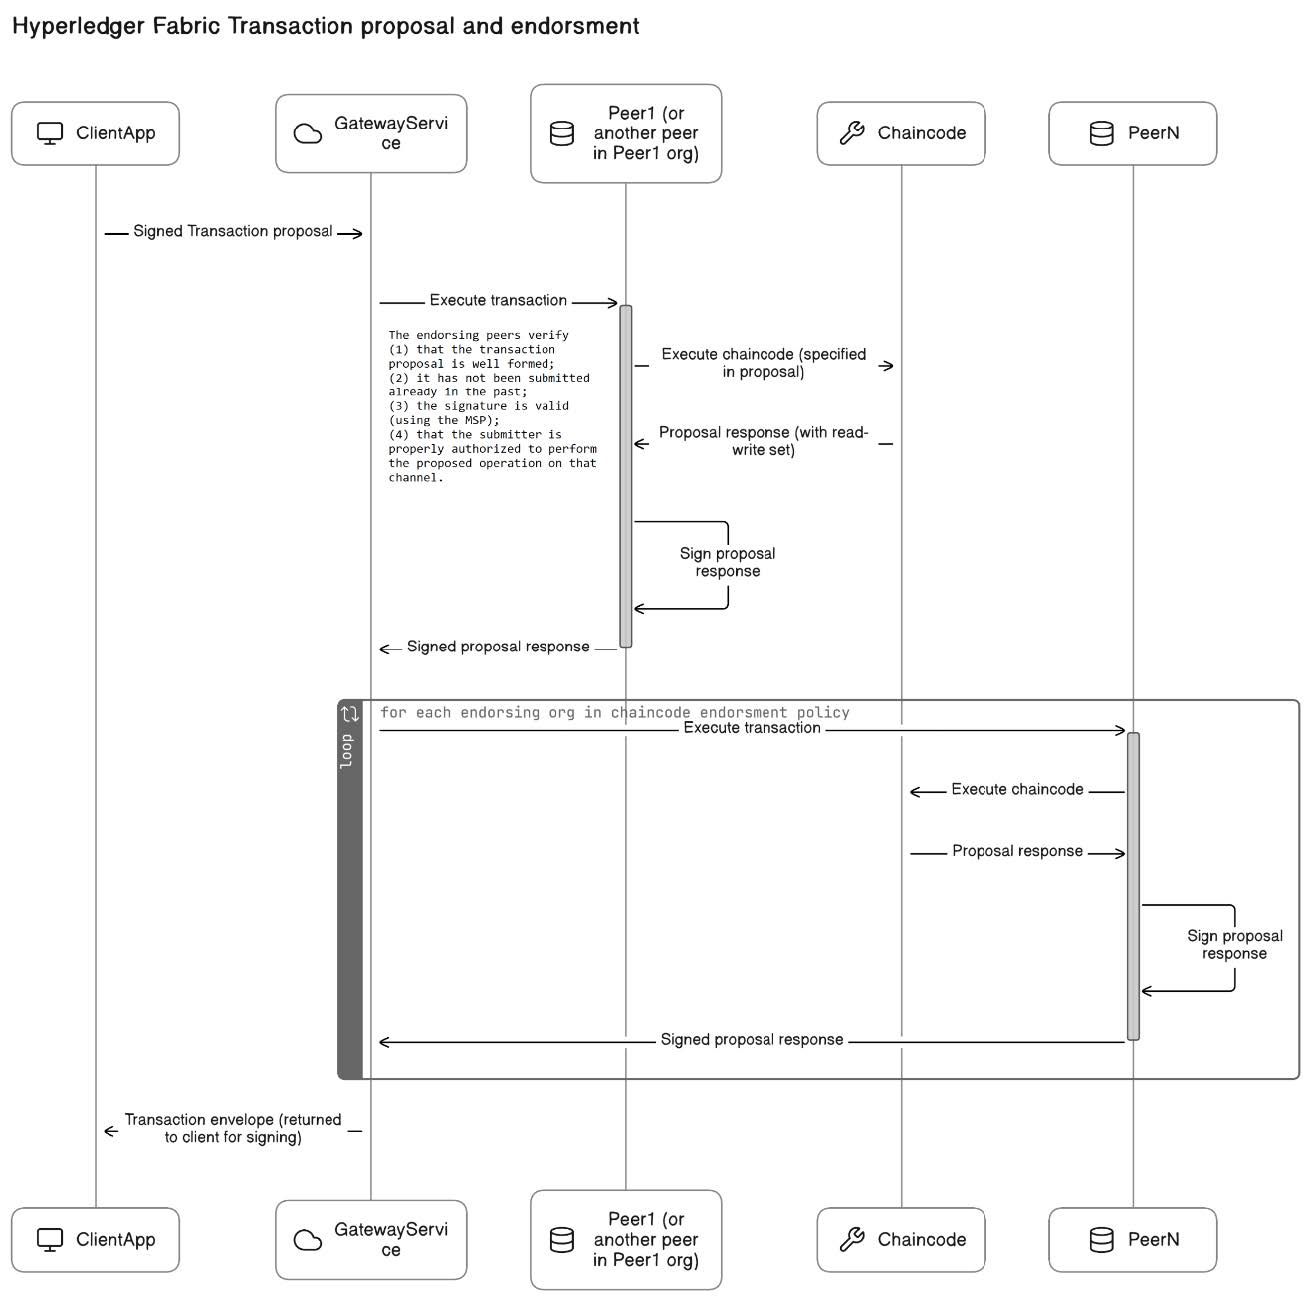
\includegraphics[width=\linewidth]{Images/Transaction 1.jpg}
    \caption{Hyperledger Fabric Transaction proposal and endorsement}
    \label{fig:transaction_1}
\end{figure}

\begin{figure}
    \centering
    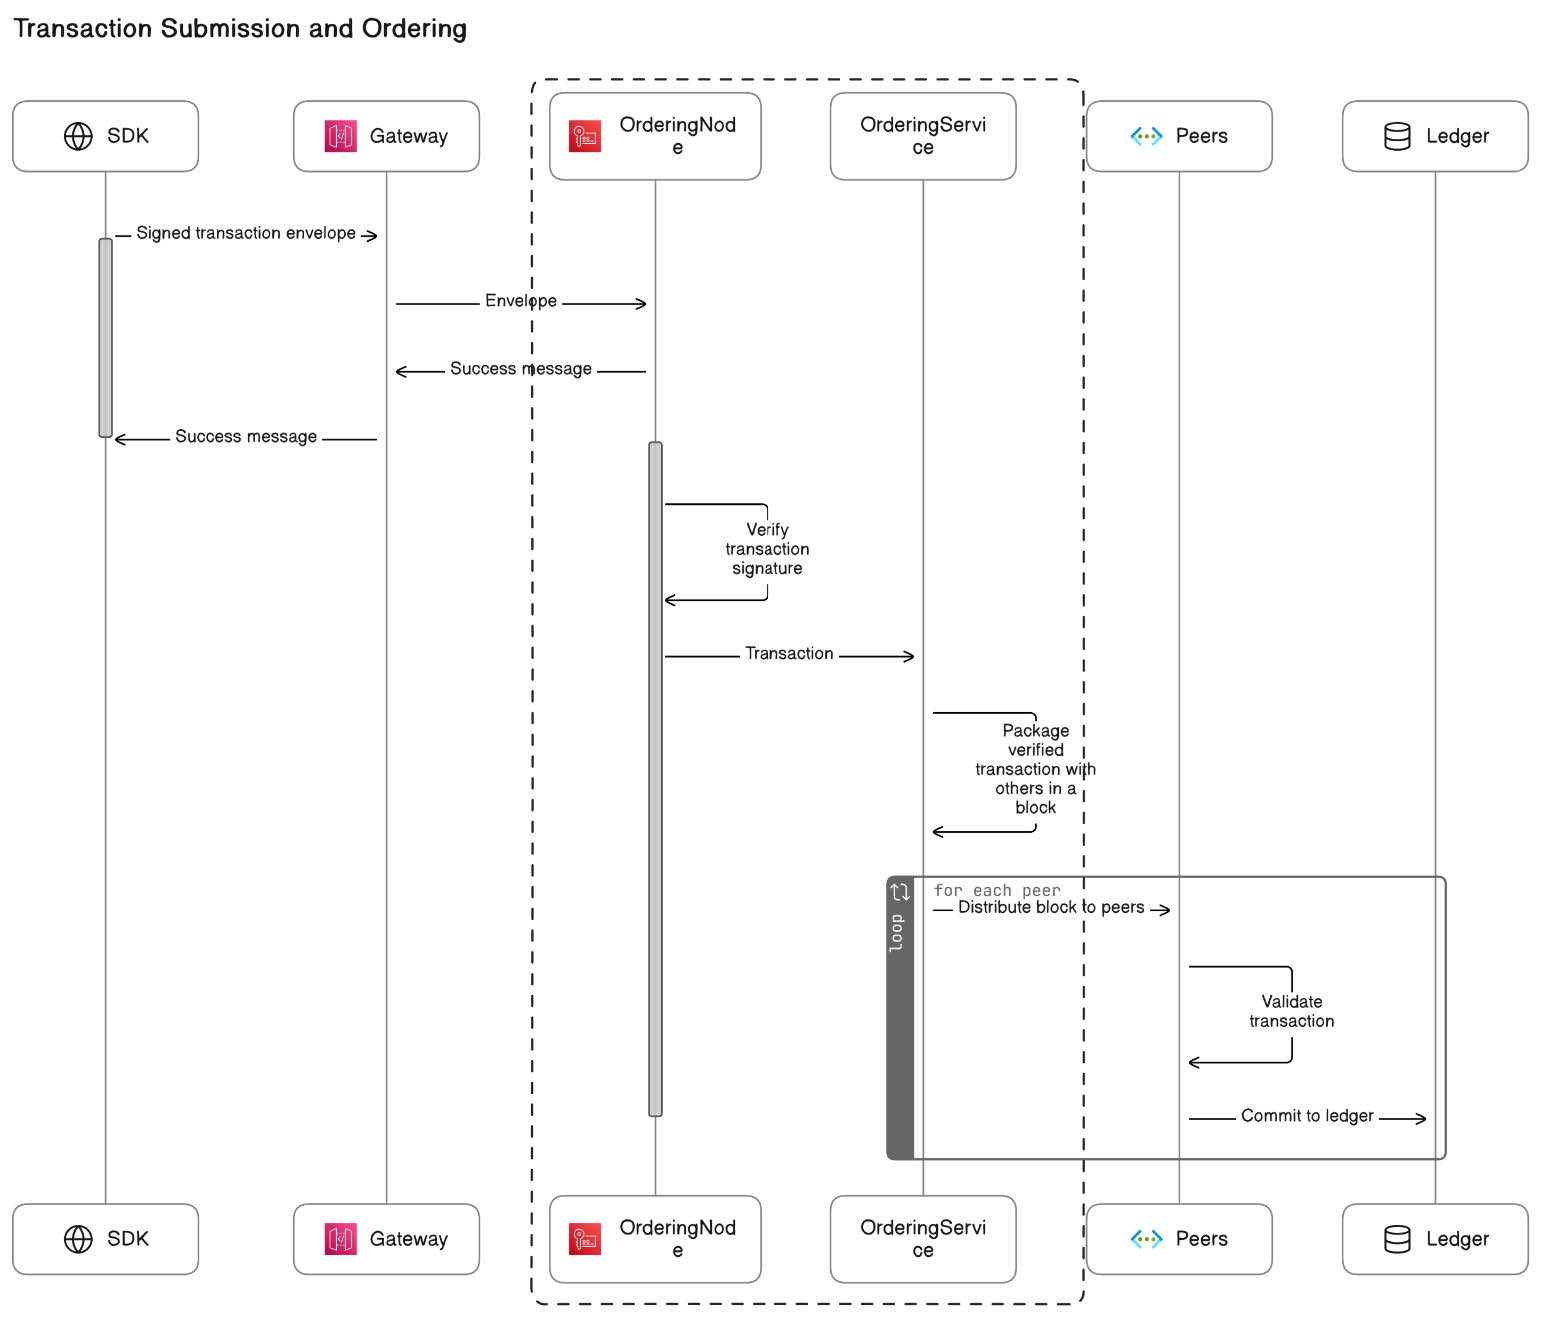
\includegraphics[width=\linewidth]{Images/Transaction 2.jpg}
    \caption{Transaction submission and ordering}
    \label{fig:transaction_2}
\end{figure}

\begin{figure}
    \centering
    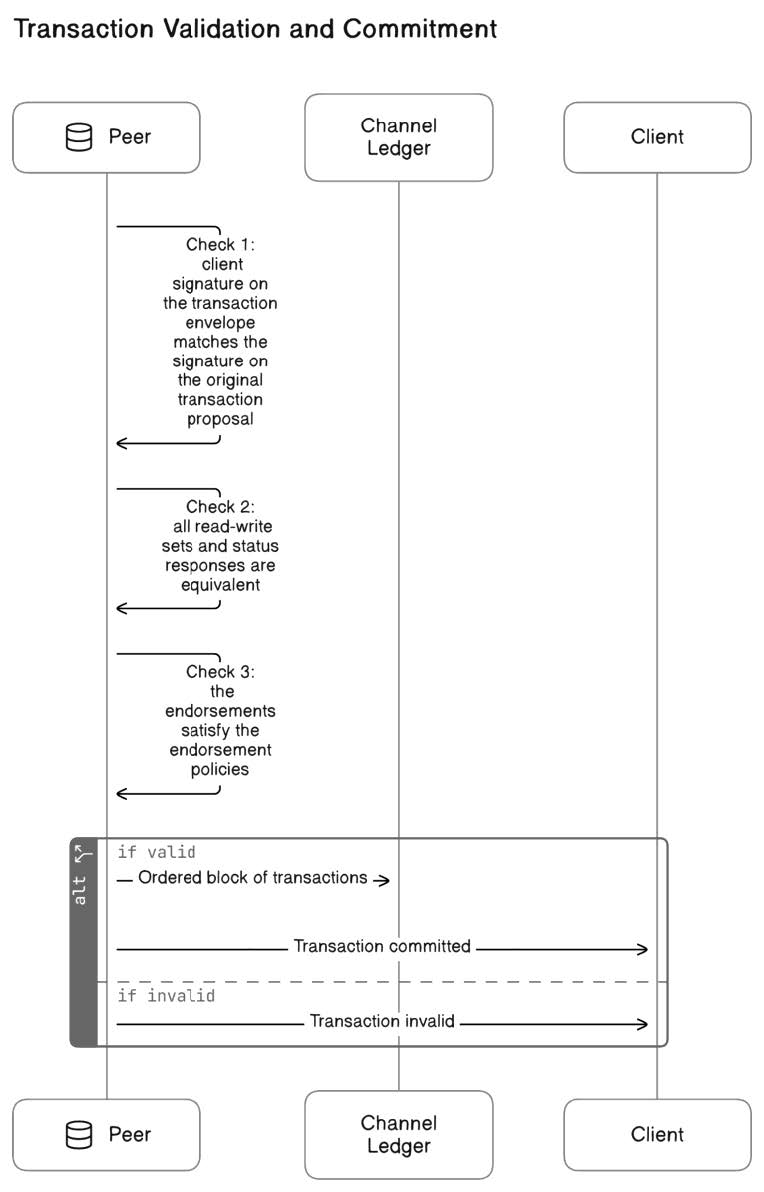
\includegraphics[width=0.9\linewidth]{Images/Transaction 3.jpg}
    \caption{Transaction validation and commitment}
    \label{fig:transaction_3}
\end{figure}

The transaction flow in Hyperledger Fabric (from version 2.4 onward, using the Gateway service) is a multi-step process that ensures integrity, authentication, and consensus.

\begin{enumerate}
    \item \textbf{Proposal Submission:} An authenticated client application creates a transaction proposal, which includes the function to be invoked on the chaincode. The client signs this proposal with its cryptographic credentials and submits it to a Gateway service running on a peer (beginning of figure \ref{fig:transaction_1}).
    
    \item \textbf{Endorsement Simulation:} The Gateway forwards the proposal to the endorsing peers as required by the chaincode's endorsement policy. Each peer verifies the proposal (signature validity, authorization, correctness) and, if valid, simulates the transaction by executing the chaincode. This produces a signed proposal response containing the read/write set.
    
    \item \textbf{Response Aggregation and Transaction Assembly:} The Gateway collects the signed proposal responses from all endorsing peers. If the responses are consistent and satisfy the endorsement policy, the Gateway assembles them into a transaction envelope, which includes the original proposal and all endorsements.
    
    \item \textbf{Transaction Submission:} The Gateway returns the prepared transaction to the client application, which signs the transaction envelope and submits it back to the Gateway (end of figure \ref{fig:transaction_1} and beginning of figure \ref{fig:transaction_2}). The Gateway then forwards the transaction to the Ordering Service.
    
    \item \textbf{Ordering:} The Ordering Service receives transactions from multiple clients across the channel, orders them, and groups them into blocks.
    
    \item \textbf{Block Dissemination:} The Ordering Service distributes the created block to all peers participating in the channel. At this stage, the service may acknowledge receipt of the transaction, but no final validation has yet occurred.
    
    \item \textbf{Validation and Commitment:} Each peer validates every transaction in the received block by performing the following checks (see the loop in figure \ref{fig:transaction_2} and figure \ref{fig:transaction_3}):
        \begin{enumerate}[label=\Roman*.]
            \item Verifying the client's signature on the transaction envelope;
            \item Confirming that the read/write sets are consistent across endorsing peers;
            \item Ensuring the endorsements satisfy the chaincode's endorsement policy.
        \end{enumerate}
    Valid transactions are committed to the ledger: the write set is applied to the world state and the block is appended to the blockchain. The client is then notified of the final outcome of the transaction. In case of invalid transactions, instead, they are not committed to the ledger and the client is notified about the invalidity of the transactions.
\end{enumerate}

This structured, multi-stage process highlights the robust security and consensus model of Hyperledger Fabric. We now turn our attention to IOTA, a DLT with a fundamentally different architecture designed for a completely different set of challenges.

\chapter{IOTA: A Distributed Ledger for the Internet of Things}

IOTA is a distributed ledger technology specifically conceived to address the inherent limitations of traditional blockchains within the Internet of Things (IoT) ecosystem. Its design goals are centered on creating a lightweight, highly scalable, and entirely fee-free environment suitable for the massive volume of micro-transactions and data transfers generated by IoT devices.\\

The IOTA whitepaper identified two primary challenges in traditional blockchain technology that it aimed to solve:

\begin{itemize}
    \item \textbf{Transaction Fees:} In use cases involving micro- and nano-payments, the transaction fee on a conventional blockchain can often be higher than the actual value being transferred. This economic barrier makes traditional blockchains impractical for many IoT applications.
    
    \item \textbf{Participant Roles:} Traditional blockchains create a distinction between users who issue transactions and a smaller group of specialized participants (miners or validators) who are incentivized to approve them. This can create bottlenecks and centralizing tendencies.
\end{itemize}

\section{The Tangle: A Directed Acyclic Graph (DAG)}

At the heart of IOTA is its core data structure, the \textbf{Tangle}, which is a Directed Acyclic Graph (DAG). Unlike a blockchain, the Tangle has no blocks; the graph is composed solely of individual transactions.\\

The fundamental mechanic of the Tangle is elegantly simple: to issue a new transaction, a user or device must first choose and approve two previous transactions. This approval process involves implicitly checking that the chosen transactions are not in conflict with each other. Some transactions can be left out and become orphaned.\\

This small amount of work performed by every participant who issues a transaction completely replaces the need for dedicated miners and, consequently, eliminates transaction fees.\\

Because there is no mining process, all IOTA tokens were created in the genesis transaction. These tokens are now in circulation, and no new tokens will ever be generated.

\section{Core Concepts and Definitions}

The IOTA Tangle is described using a specific set of terminology that defines its structure and operation.

\begin{itemize}
    \item \textbf{Vertex:} A single transaction within the Tangle.
    \item \textbf{Edge:} A directed link from one transaction (A) to another (B), signifying that transaction A approves transaction B. If there is a path from A to C of length > 1, then A indirectly approves C.
    \item \textbf{Weight:} A numerical value representing a transaction's importance. The IOTA whitepaper defines this value as $w = 3^n$, where $n$ is a non-negative integer.
    \item \textbf{Tip:} A transaction in the Tangle that has not yet been approved by any other transaction. New transactions are typically attached to tips.
    \item \textbf{Cumulative Weight:} The sum of a transaction's own weight plus the sum of the weights of all transactions that directly or indirectly approve it. This serves as a measure of a transaction's confirmation level.
    \item \textbf{Height:} The length of the longest path from a transaction back to the genesis transaction.
    \item \textbf{Depth:} The length of the longest path from a transaction forward to a tip.
\end{itemize}

\section{The Transaction Approval Process: Tip Selection Strategies}

The strategy used by nodes to select which "tips" to approve is critical for maintaining the health, security, and forward momentum of the Tangle. A well-designed tip selection algorithm encourages the network to grow in a consistent and secure manner, while a poor one can introduce significant vulnerabilities.

\subsection{Random Tip Selection}

This initial approach allows a user to approve any two tips chosen at random. However, this method has notable weaknesses. It allows "lazy nodes" to approve very old transactions, which does not contribute to confirming recent activity. Furthermore, it enables "malicious nodes" to artificially inflate the number of tips by issuing transactions that approve the same fixed pair, undermining the network's intended structure.

\subsection{MCMC (Markov Chain Monte Carlo)}

This strategy provides a more robust and secure mechanism for network growth by guiding nodes to approve more recent and heavily-weighted tips. The algorithm initiates multiple "random walks" starting from the Genesis transaction and traversing the graph probabilistically toward the tips. The tips most frequently reached across these walks are selected for approval. By probabilistically favoring paths with higher cumulative weight, the MCMC algorithm inherently guides new transactions to approve the tips that are part of the most trusted and active section of the Tangle. This directly counters the "lazy node" problem by making it computationally unlikely for a random walk to terminate at a stale, old tip, and it discourages malicious tip inflation by concentrating confirmation weight on the main, honestly growing part of the graph.

\section{MCMC Transition Probability}

The MCMC strategy relies on a probabilistic model to guide the random walks. The probability of transitioning from transaction \textit{x} to an adjacent transaction \textit{y} at each step of the walk is proportional to the following formula:

\begin{center}
    $e^{-\alpha(H_x - H_y)}$
\end{center}

Where:
\begin{itemize}
    \item \textit{\textbf{H}} is the cumulative weight of a transaction.
    \item \textit{\textbf{$\alpha$}} is a chosen tunable parameter greater than zero.
\end{itemize}

This formula's effectiveness lies in the difference between the cumulative weights ($H_x - H_y$). If a potential next transaction \textit{y} has a much higher cumulative weight than the current transaction \textit{x}, the exponent becomes a large positive number, making the transition probability very high. Conversely, a move to a "weaker" transaction with a lower cumulative weight is heavily penalized, effectively steering the selection process toward the most heavily confirmed parts of the Tangle. This process of validation is complemented by a mechanism designed to prevent network spam.

\subsection{Example of tangle and MCMC random walks}

\begin{figure}
    \centering
    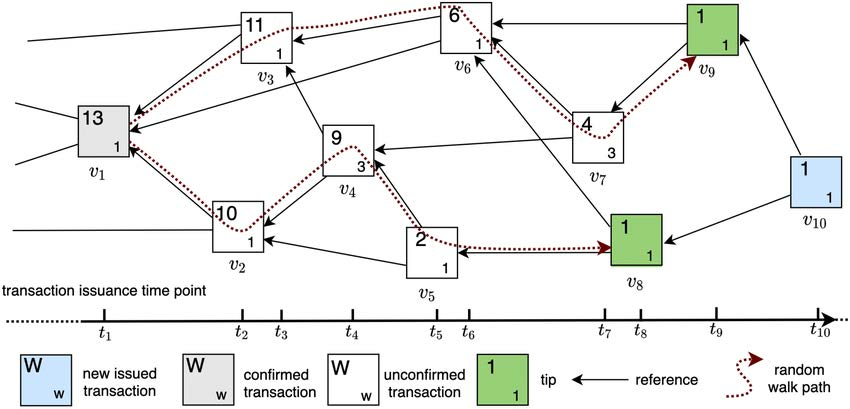
\includegraphics[width=\linewidth]{Images/Tangle.jpg}
    \caption{Example of tangle and MCMC random walks}
    \label{fig:tangle}
\end{figure}

Figure \ref{fig:tangle} shows an example of the Tangle and two random walks starting from a confirmed transaction. In IOTA, a transaction is considered \textbf{confirmed} (i.e., final) when it is directly or indirectly approved by a \textit{milestone} issued by the Coordinator. Therefore, confirmation does not depend on reaching a specific cumulative weight threshold, but on the presence of a milestone approving the transaction.\\

Each transaction in the Tangle is associated with two weights. The smaller value (shown in the bottom-right corner) is the \textbf{own weight} of the transaction, defined as $w = 3^n$, where $n$ is a non-negative integer. The larger value (shown in the top-left corner) is the \textbf{cumulative weight}, defined as the sum of the weight of the transaction itself and the weights of all transactions that directly or indirectly approve it.\\

The computation of cumulative weights requires traversing the Tangle as a directed acyclic graph (DAG). In particular, care must be taken to avoid counting the same transaction multiple times when multiple paths exist (for instance $v1$ is approved by $v6$ both directly and indirectly through $v3$). For this reason, the cumulative weight is not simply the sum of the cumulative weights of the direct approvers. In practice, nodes compute (and possibly cache) cumulative weights locally; there is no global shared state that is updated when new transactions are added.\\

When a node wants to issue a new transaction (e.g., $v10$), it must approve exactly two previous transactions, called \textbf{tips} (i.e., transactions that have not yet been approved). This is a mandatory requirement of the protocol and does not provide any reward or token that can be accumulated: each new transaction must perform this approval step.\\

The selection of the two tips is performed using a \textbf{Markov Chain Monte Carlo (MCMC)} algorithm. This consists of executing two independent random walks starting from a sufficiently deep (and typically confirmed) transaction and moving toward the tips. This algorithm biases the walk toward transactions with higher cumulative weight, while still allowing occasional selection of lower-weight transactions.\\

Let us consider the two random walks shown in the figure: Starting from the initial confirmed transaction, the algorithm probabilistically selects among its approvers, favoring those with higher cumulative weight. This explains why, in the example, transactions with higher cumulative weights are more likely to be chosen, although lower-weight choices may still occur due to the stochastic nature of the algorithm.\\

Following the first walk, the algorithm eventually reaches a tip (e.g., $v9$), which becomes the first selected transaction to approve. The second random walk proceeds independently and may take a different path, again guided by probabilistic choices influenced by cumulative weights. Due to the stochastic nature of the process, the algorithm may occasionally select a less likely branch.\\

It is important to note that the two random walks are independent and based only on the local view of the Tangle maintained by the node. The algorithm does not perform global reasoning about previously selected paths and does not attempt to avoid selecting the same tip in advance. If both walks happen to select the same tip, the selection is considered invalid, and the node simply repeats the process (typically re-running one of the walks) until two distinct tips are obtained.\\

Once two valid tips have been selected, the node can issue the new transaction (e.g., $v10$), which will approve those two transactions and be added to the Tangle.

\section{IOTA's Proof-of-Work: A Mechanism for Spam Prevention}

The concept of Proof-of-Work (PoW) in IOTA serves a purpose that is entirely distinct from its role in other cryptocurrencies. In IOTA, PoW is not a consensus algorithm used to select a leader or "miner" to create a new block. Instead, it functions purely as a spam prevention mechanism.\\

To issue a valid transaction, a node must solve a relatively simple cryptographic problem. While this PoW is less computationally demanding than that required for Bitcoin mining, it is still expensive enough to make it infeasible for malicious actors to flood the network with spam transactions or execute Sybil attacks by creating numerous fake identities. Every transaction must include proof of this computational work—a hash that satisfies a certain difficulty level. IOTA nodes have flexibility in how they handle this requirement.

\begin{itemize}
    \item \textbf{Local Computation:} This option requires no trust in external parties, as the work is performed directly on the user's device. However, it demands higher local computing resources.
    \item \textbf{Remote Node Computation:} A user can delegate the PoW to a remote node. This requires trusting the remote node to perform the computation correctly and return the result. It also introduces potential issues such as connection latency or timeouts if the remote node is overloaded with requests.
    \item \textbf{Outsourced Paid Service:} For users seeking greater efficiency, PoW can be outsourced to a dedicated paid service. While this option costs currency, it typically provides higher performance and reliability than other methods.
\end{itemize}

While PoW deters spam, another mechanism is currently in place to ensure the finality and definitive state of transactions on the network.

\section{Network Security and Finality: The Role of the Coordinator}

In its current stage of development, the Tangle architecture is vulnerable to certain large-scale threats, specifically Sybil and 34\% attacks. To mitigate these risks and guarantee transaction finality, the IOTA network employs a special node known as the Coordinator.

\subsection{Coordinator Functionality}

The Coordinator is a centralized node run by the IOTA Foundation and hardcoded into the IOTA Reference Implementation (IRI). Its primary function is to periodically (approximately every minute) issue special zero-value transactions, called \textit{milestones}. These milestones act as checkpoints that provide finality to the Tangle.\\

A transaction is considered \textbf{final} when it is directly or indirectly approved by a milestone. Direct approval occurs when the milestone explicitly references a transaction. Indirect approval arises from the structure of the Tangle: if a milestone approves a transaction $A$, and $A$ directly or indirectly approves other transactions (e.g., $B$ and $C$), then the milestone also indirectly approves $B$ and $C$. Therefore, each milestone confirms an entire subgraph of transactions reachable by traversing the Tangle backward from the milestone.\\

The Coordinator does not maintain a global queue of transactions waiting for confirmation. Instead, it selects transactions using a strategy similar to the MCMC-based tip selection algorithm, typically favoring recent transactions that are well integrated into the Tangle.\\

An important consequence of the DAG structure is that a single milestone can confirm a large number of transactions at once. Since each approved transaction recursively approves many others, the confirmation propagates backward through the graph. For this reason, the Coordinator does not need to directly approve every transaction individually.\\

In practice, this leads the Coordinator to select transactions that are not too deep in the Tangle (i.e., relatively close to the current frontier of unconfirmed transactions). By approving such transactions, the milestone indirectly confirms a large portion of the Tangle, including many older transactions that lie in their past cone. This makes the confirmation process efficient even when the rate of transaction issuance is much higher than the rate of milestone creation.\\

As a consequence, confirmation is an emergent process. Transactions that are well-integrated into the Tangle are more likely to be indirectly confirmed by future milestones, while transactions that remain weakly connected may never be confirmed and can eventually become orphaned.\\

In this sense, milestones do not confirm individual transactions in isolation, but rather stabilize entire regions of the Tangle, progressively extending the portion of the graph that is considered definitive.

\subsection{A Temporary Measure}

It is critical to note that the Coordinator is explicitly designed as a temporary security measure. The IOTA Foundation's objective is to decentralize the network fully once it achieves a sufficient level of organic activity and security. The Coordinator will become unnecessary and will be removed from the network when the network size and the rate of transactions per second increase to a point where the Tangle is robust enough to resist attacks on its own.\\

In summary, the IOTA Tangle's DAG-based architecture represents a fundamental innovation in distributed ledger design. While pragmatic, centralized measures like the Coordinator are currently employed to bootstrap network security, the protocol's core design principles are aimed at achieving a fully decentralized, scalable, and self-sustaining ecosystem.

\end{document}
